\section{Domain Analysis}
\phantomsection

\subsection{REST}
REST (Representational State Transfer) relies on a stateless, client-server architecture that uses the HTTP protocol in the most cases.
REST is an architecture style used in the development of Web services. Instead of using complex mechanisms such as CORBA, RPC or SOAP to connect between devices, REST is preffered as a way for the devices to communicate.
REST uses HTTP for the CRUD (Create/Read/Update/Delete) operations.
As a programming approach, REST is a lightweight alternative to Web Services.
A REST service is:
\begin{itemize}
  \item Does not depend on platforms (the server can be Unix, Mac or any other kind)
  \item Based on standards (runs on top of HTTP)
  \item Is not language dependent(Java can communicate with Python)
  \item Can be easily used if there are firewalls present
\end{itemize}

There are six constraints which describe the REST architecture. Five of them are mandatory. If the system doesn't comply with these, it cannot be considered RESTful, even though it is constructed in a RESTlike way.
These are the six constraints that define the RESTful architecture style:
\begin{enumerate}[label=\arabic*)]
  \item Uniform Interface

    The \textit{uniform interface} constraint simplifies and declutches the architecture into parts, which can then grow independently. It represents the interface between clients and servers. The uniform interface is an essential part of the outline of any REST services.  The rules which direct the uniform interface are:

    \begin{description}
      \item[Resource-Based] \hfill \\
        URIs are the resource identifiers, which help to detect the individual resources in a request. The resources and the representations, that are returned to the client as an answer to their request are two considered two separate things. As an example, the server sends some database records in a XML or JSON, which can be expressed in different languages and encodings, based on the server implementation and the particularity of the received request, instead of sending its database.

      \item[Manipulation of Resources Through Representations] \hfill \\
        If a client has the permission to modify or delete a resource on the server, he can do so, given he has a representation of that resource and the metadata it holds, if any.

      \item[Self-descriptive Messages] \hfill \\
        Messages must contain sufficient information, so the hosts know how to process them. Given a media type in the message, the host will choose the necessary parser to operate on the contents of it. Responses must explicitly mention if they are cacheable.

      \item[Hypermedia as the Engine of Application State (HATEOAS)] \hfill \\
        State is delivered between hosts via hypermedia. Clients provide state through body contents, query parameters, request headers and the resource name (URI). Servers endow state to clients via response codes, headers and body content.
        HATEOAS also expresses the possibility of placing the URI in the body or header of the response to provide the resource name for the recovery of the relevant objects.
    \end{description}

  \item Stateless

    The \textit{statelessness} of the REST architecture signify that the request contains the required state, which is used to deal with the request itself.
    It can be inside the URI, query-string parameters, body or headers. The resource is identified by the URI and its state is found in the body. The request is analized and processed by the server and then the according state is transmitted back via response body, headers.
    In REST, the server does not have to preserve, update or transmit the session state, thus allows more scalability. Session state is stored fully on the client. The client must contain in the request all the information for the server, so it can be performed. Also including state if it should spread more requests.

    The application state is the data used for the current session or request by the server, to carry out a request. A resource is the data that represents the resource description, which can be the data that is stored in the database. The application state can differ per request and client, where the resource state remains the same for every client that sends a request for it.

    This constraint establishes visibility, reliability, and scalability. The system doesn't have to look at anything else besides the request itself to identify the character of the request, thus improving visibility. The recuperation from small errors is easier, making the system more reliable. The server doesn't need to administer resource usage of requests and to store state from requests, which makes the system easier to maintain and develop.

  \item Cacheable

    The clients must have the possibility to \textit{cache} responses. To avert clients reutilizing outdated or deficient data in requests, the responses must declare themselves as cacheable or non-cacheable. Scalability and performance can be enhanced, when caching is adequately managed, thus decreasing certain client-server communication and reducing the average latency. 

  \item Client-Server

    \textit{Clients and servers} are divided by the uniform interface. This means that the portability of the client code can be increased by leaving, for example, the data storage to the responsibility of the server, making the client unrelated dircectly with the storage mechanism. Servers also are improved by this splitting by making it ignorant to the user state or interface, thus making them more intelligible and scalable. Given that the interface is not intefered with, servers and clients can be extended and changed without taking care of any diret relation between them.

  \item Layered System

    Intermediary serevers are used in a \textit{layered system}. They can improve the system's scalability by using load-balancing of services between multiple networks and shared caches. Also, the security can be strenghtened by the use of layers. Clients should not be able to differentiate whether it is connected directly to the server it is accessing or to an intermediate server.
    The downside of a layered system is that it can generate overhead and latency to the data processing. If it is supports cache contstraints, then it can profit from the shared caching at intermediary servers.

  \item Code on Demand (optional)

    The functionality of the client side can be enhanced by providing executable logic by the servers. The amount of features to be implemented at client-side drops thanks to this constraint. System extensibility is improved by having the opportunity to download additional features to the system.

\end{enumerate}

If we support these constraints, we get the following possibilities inside our system:
\begin{itemize} 
  \item Scalability
  \item Simplicity
  \item Modifiability
  \item Visibility
  \item Portability
  \item Reliability
\end{itemize}


\subsection{Rails}

Rails is a web-application framework that includes all necessary to create web applications fitting to the Model-View-Controller (MVC) pattern.
MVC pattern comprehension is essential to understanding Rails, so MVC will be described further.
MVC splits your application into three layers, each having a distinctive duty.

The Model layer depicts your domain model and contains the business logic that is individual to your application. ActiveRecord::Base is the class from which the database-backed model classes are inherited, in Rails. Data from database tuples are given as objects which have business logic methods, thanks to Active Record. Models can be ordinary Ruby classes, or classes that apply a set of interfaces as given by the Active Record module, while most Rails models are supported by a database.

Incoming HTTP requests and the appropriate responses for them are managed by the Controller layer.
Rails controllers can generate HTML, XML, JSON, mobile views, PDFs as returning response to the request. Controllers render view templates and control the models so that it can give a suitable HTTP response. 

Action Dispatch parses the web request's contained information routes the requests to the right controller and deals with advanced processing connected to HTTP:
\begin{itemize}
  \item MIME-type negotiation
  \item Decoding parameters in PUT, PATCH and POST
  \item Control HTTP caching, cookies and sessions
\end{itemize}

Controller classes inherit from the ActionController::Base class and implement actions to manage requests. The content which is generated from views is usually what is displayed as the result of an action. 

In Rails framwork, the Action Dispatch functionality is dispatched by default, and the users interface with the Action Controller module, which prompts the Action View rendering. 

Action Pack contains both Action Dispatch and Action Controller modules. So it provides both the view and the controller layers of the MVC. Action Pack is a framework that manages web requests. With it, you can route (map the request URLs to their respective actions), establish controllers which apply actions, and render views(templates of different formats) as responses.


``Templates'' are the essential part of the View layer and they are the ones that deliver the  proper representations of the app's resources. The most frequent view temlates are ERB files, which are HTML with embedded Ruby, though they can be found in diverse formats. Action View manages the view generation. A controller response or some text is usually rendered in a view.
 
Rails also has Action Mailer, used to generate and send emails; Active Job, an interface used to put different jobs to run on background using one of the queueing backends; Active Support, a module offering library extensions and utility classes.

\subsection{Quick Response Codes}
The QR code, which stands for Quick Response Code, is a two-dimensional barcode, which was initially used for tracking inventory. It was developed in Japan by a subdivision of Toyota. Today, it is widely spread and people have found more and more uses for it. The fast gain in popularity was due to the superiority of the QR codes’ read speed and storage capacity versus the UPC barcodes.

The QR code is  composed of black square dots placed on a white square background. It is usually read by a phone camera, which has a QR decoding software. The code image is then interpreted and the data is extracted.

The code can be read from any direction in 360 degree. The three corners of the QR code contain the positional detecting patterns, which make this thing possible.

\subsubsection{QR Error Correction}
The QR error correction is used to restore the data on a damaged code. There are four levels of correction. If a higher level is set, the error correction is more efficient but less characters can be encoded. So you must be careful when deciding which error correction level to use. Most of the time, the decisive factor is the environment in which the QR codes will be used. So take the probability of the QR code to be damaged into consideration and decide about the error correction level accordingly.

\subsubsection{QR code sizes}
The black dots in the code are also called modules. Their size are an important factor that categorize the QR codes in readable and not readable by certain devices. The QR codes become unreadable if their modules’ size are below the resolution limitation of the imaging device’s camera.

The QR code is designed in such a way that, the more data you want to store in it, the more columns and rows containing modules will be inserted. Therefore, a QR code must have a bigger size when a larger amount of data is encoded and vice-versa.

So, the QR codes have been categorized in versions, from Version 1 to Version 40.  QR code Versions differing from the previous one by having 4 more modules on each side: Version 1 with ( 21 x 21 modules ) with possibility of storing 25 alphanumerics with the lowest correction level and Version 40 with  ( 177 x 177 modules ) with 1852 alphanumerics. The maximum data storage for each version is derived from the amount of data, character type and correction level.


\begin{figure}[!ht]
  \centering
  \subfloat[Version 1 QR code\label{fig1.1a}]{%    
    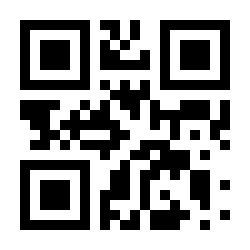
\includegraphics[width=0.48\textwidth,natheight=292, natwidth=292]{qr_v1.png}    
  }
 \hspace{0.09cm}
  \subfloat[Version 40 QR code\label{fig1.1b}]{%
    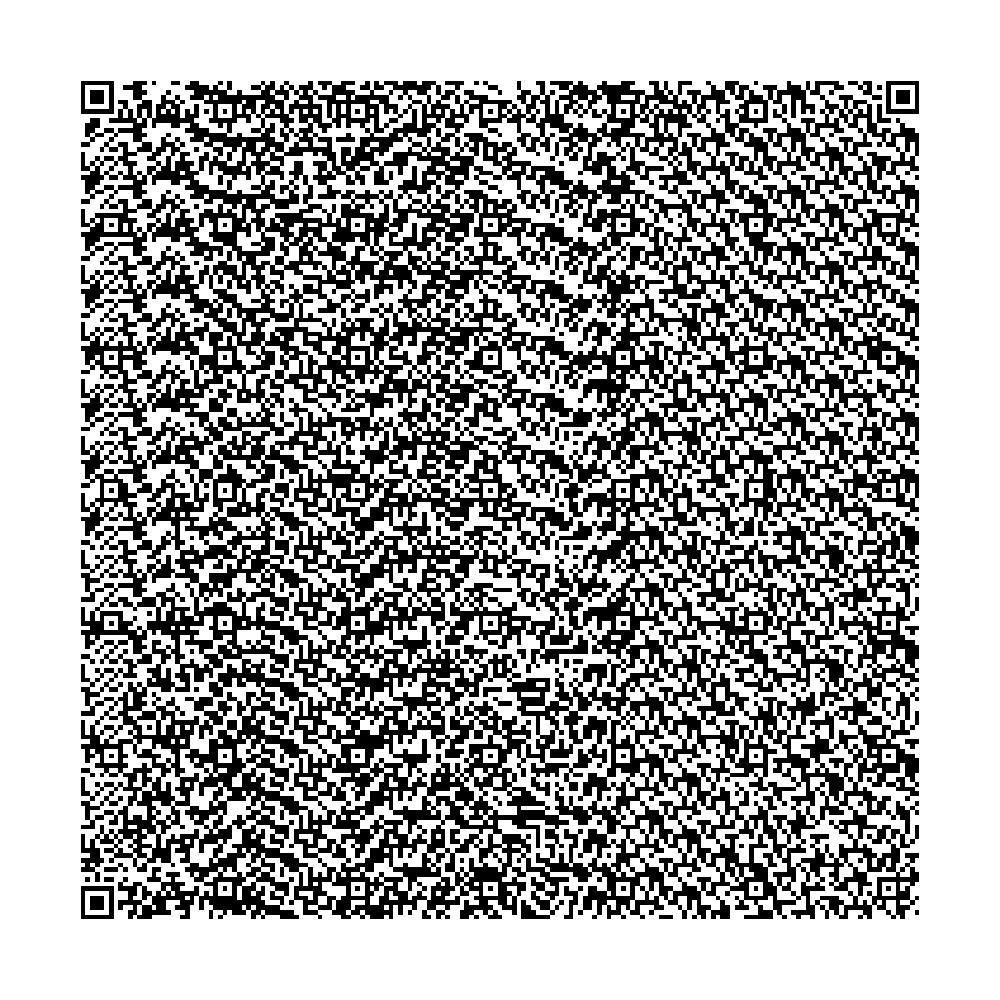
\includegraphics[width=0.48\textwidth,natheight=1000, natwidth=1000]{qr_v40.png}
  }
  \caption{Version 1 QR code with 21 x 21 modules (a), version 40 QR code with 177 x 177 modules (b).}
  \label{fig1.1}
\end{figure}



Having this technology at hand, the system gets to simplify the way in which it recognizes the different pages it is processing at the low level of its implementation. Given that information being stored in the QR code will be minimal, it is not required a size bigger than the Version 1 provides us, thus saving some space on the printed paper. The correction level will be set to high, for safety reasons and also because it won’t conflict with the number of characters needed to be encoded.

\clearpage

